\documentclass[../piano-di-progetto.tex]{subfiles}

\begin{document}

  \subsection{Progettazione di dettaglio e codifica}

  \subsubsection{Prospetto orario}
  Nel periodo di Progettazione di dettaglio e codifica, la distribuzione oraria è la seguente:
  \begin{table}[H]
    \centering
    \begin{tabular}{lccccccc}
      Nominativo                & Re          & Am          & An          & Pt           & Pr           & Ve          & Ore totali   \\
      Sofia Bononi              & 7           & -           & 4           & 14           & 17           & 12          & 54           \\
      Enrico Buratto            & -           & 4           & -           & 15           & 22           & 13          & 54           \\
      Ian Nicolas Di Menna      & -           & 7           & -           & 15           & 17           & 16          & 55           \\
      Alessandro Franchin       & -           & 4           & -           & 14           & 22           & 13          & 53           \\
      Enrico Galdeman           & -           & 5           & 4           & 13           & 17           & 13          & 52           \\
      Nicholas Miazzo           & 6           & -           & 4           & 15           & 15           & 15          & 55           \\
      Marco Nardelotto          & 7           & -           & -           & 16           & 16           & 14          & 53           \\
      \textbf{Ore totali ruolo} & \textbf{20} & \textbf{20} & \textbf{12} & \textbf{102} & \textbf{126} & \textbf{96} & \textbf{376}  
    \end{tabular}
    \caption{Distribuzione oraria del periodo di Progettazione di dettaglio e codifica}
  \end{table}


  Per facilitare la lettura della distribuzione oraria, i dati vengono rappresentati graficamente il seguente istogramma:
  \begin{figure}[H]
    \centering
    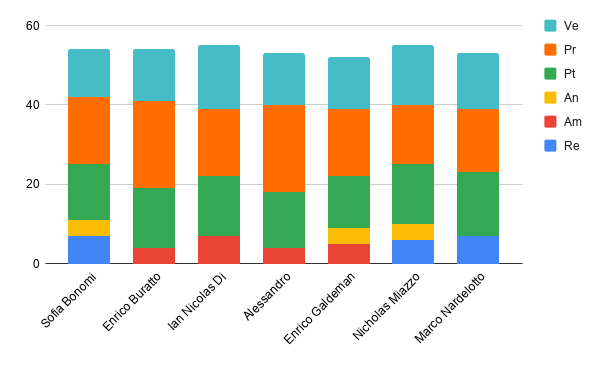
\includegraphics[width=12cm]{img/ore-codifica.png}
    \caption{Istogramma della distribuzione oraria del periodo di Progettazione di dettaglio e codifica}
    \label{fig:ore-componente-codifica}
  \end{figure}

  \subsubsection{Prospetto economico}
  In questo del periodo, la suddivisione oraria e i costi per ruolo è la seguente:

  \begin{table}[H]
    \centering
    \begin{tabular}{lcc}
      Ruolo           & Ore previste & Costo               \\
      Responsabile    & 20           & € 600,00            \\
      Amministratore  & 20           & € 400,00            \\
      Analista        & 12           & € 300,00            \\
      Progettista     & 102          & € 2.244,00          \\
      Programmatore   & 126          & € 1.890,00          \\
      Verificatore    & 96           & € 1.440,00          \\
      \textbf{Totale} & \textbf{376} & \textbf{€ 6.874,00}
    \end{tabular}
    \caption{Prospetto economico del periodo di Progettazione di dettaglio e codifica}
  \end{table}


  Per facilitare la lettura della suddivisione oraria per ruolo, i dati vengono rappresentati graficamente mediante il seguente areogramma:
  \begin{figure}[H]
    \centering
    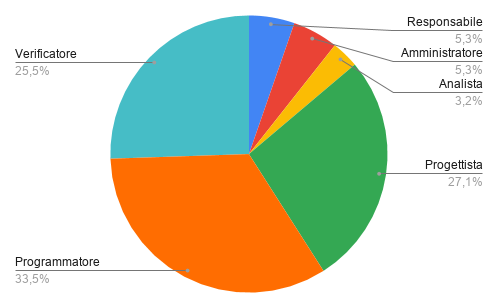
\includegraphics[width=12cm]{img/ruoli-codifica.png}
    \caption{Areogramma della suddivisione dei ruoli del periodo di Progettazione di dettaglio e codifica}
    \label{fig:ore-ruolo-codifica}
  \end{figure}

\end{document}
